
In this chapter, the results and other constraints encountered will be discussed.

\section{Project Management}

Early in the planning and management phase of this thesis, it became evident that the Norwegian infrastructure for retrieving data from various public sources by API was not sufficient for the needs of this thesis. Therefore the initial plan to automate the collection of data needed was adapted to the means of acquiring the data by manually asking the various agencies and implementing their data hard-coded. This makes the program much less scalable and flexible than hoped for, and severely inhibits future contributions as it may be difficult to couple new data with the inputs of the backend's data structure. The missing automation part will probably hinder future use of this program. The only two APIs used are of American origin, namely Google static map and Twitter. In these regards the automation element that this thesis anticipated failed, however not by a critical means as manual retrieval of data was still possible.






\section{Project resolutions}
In the middle of the time scope for this thesis, a frontend to the backend was desired and thus planning to construct this began. There were several options for choosing not only from the languages the GUI would be based upon but consideration of how a map would be projected as well. These were the main concerns and had to be compatible with each other. The first choice was between Python's Tkinter GUI module and Node/Javascript GUI. The main reason Python was chosen was that it offered the easiest integration with the backend. Javascript prohibits direct reading from local files, and thus the backend would have to be mounted on a server in order to provide its functions to a frontend. The author of this thesis had little experience with this, and learning a whole new trade was daunting and seemed insurmountable within the rest time scope of this thesis, therefore the enticing of the familiarity of Python triumphed. In hindsight, it would probably be better to undertake a Node/Javascript approach because some sort of database to store the backend's data is needed anyway and is probably a more feasible solution, more on this in the following chapter.

Choosing a map implementation was difficult, Python has several options like GeoPandas, ipyleaflet, Google static map, cartopy, OpenStreetMap, and basemap. All of the mentioned was hard to install and was sorely limited in function and potential, except OpenStreetMap and Google static map. Upon further investigation Goompy, as described in chapter 2, was discovered and offered a nearly effortless implementation of the map in the already applied design of the frontend.

The advantage the Python solution has is that it requires few installations of external modules and is easily downloaded and mountable on many platforms.
The disadvantage with Python's module Matplotlib, which is used to draw graphs, is that drawing many graphs requires a lot of memory and processor resources, therefore it is important to manage the graphs drawn, and only load those that need be loaded at a time, flushing those that are no longer in use.
The advantage of Google static map is that it is a well implemented and established service with consistent qualitative measures. Google offers fewer road details than OpenStreetMap, and that serves this thesis perfectly as the visualization needed was simply showing locations of traffic registration stations and not necessarily other roads.
The disadvantages with Google static map is that there are standard usage limits (which can simply be overcome with paying for more). Pixel resolution is set to a maximum of 640x640 pixels, and the free usage is limited to 25.000 map loads per 24 hours. These two limits are not really a problem: The pixel limit is overcome by simply requesting more map loads and then combining those to create as big a picture as desired, and the map loads limit is very high. On average Goompy does 4 map loads per zoom (thus creating a big map of 1280x1280 pixels) and 25.000 / 4 = 6250 zooms per 24 hours, average Norwegian working hours per day is 7.5 hours, this means that one would reach the limit if there are 6.250 / 7.5 / 60 = 13.9 zooms per second. This limit was never reached in testing and although it is a high limit if reached the map simply stops working for the remainder of the time to the next 24 hours. Perhaps the most severe limit Google static map have for the scope of this thesis is its maximum URL size of 8192 characters. Figure \ref{fig:google_url} show the programs URL that it sends to the Google map servers, containing a standard map and fifty-three traffic registration stations each with their individually different sizes and colors this surmounts to a total of 4.975 characters already, which is 60.7\% of the total allowed. 

\begin{figure}[h]
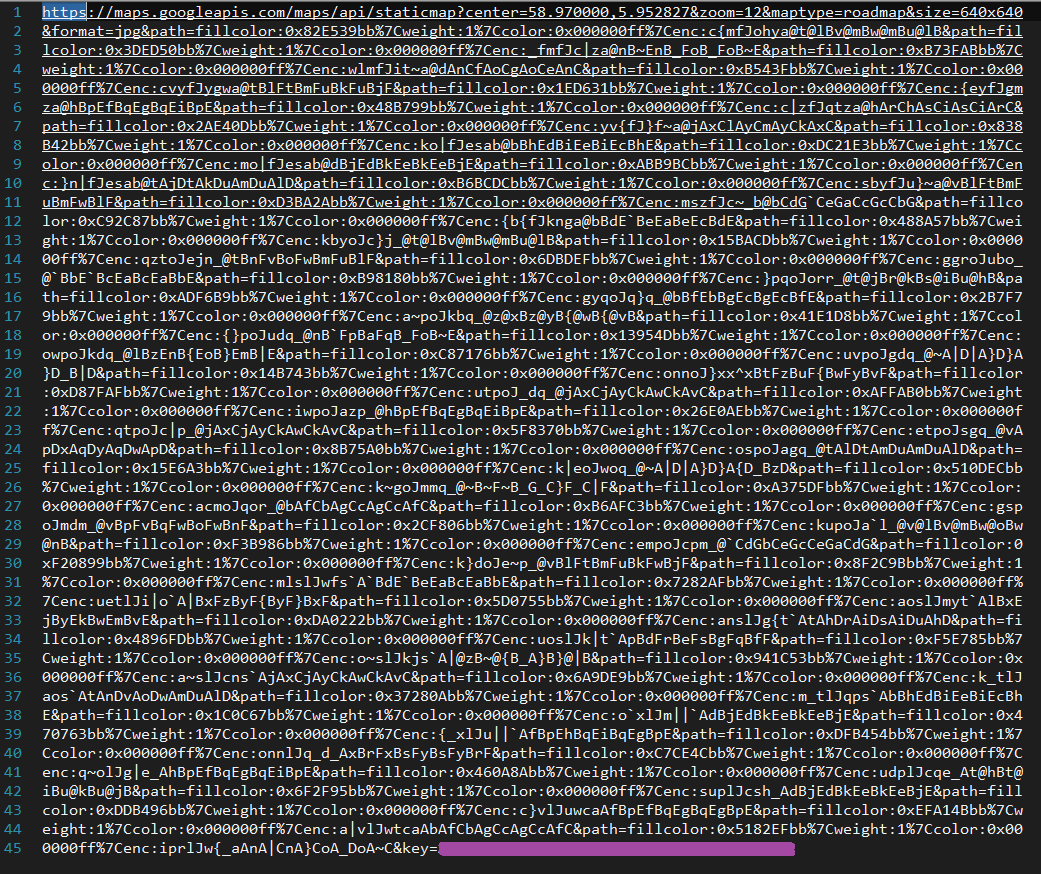
\includegraphics[width=12cm]{Google_static_map_URL}
\centering
\caption{Size of the programs Google static map URLs}
\label{fig:google_url}
\end{figure}

Although the url have encoded polylines, which compresses the data, it is already quite long, Loading all of Norway's current 10.066 traffic registration stations using Google static map with this thesis's current algorithms is not feasible, although this could be solved by clustering the traffic registration stations together, and only loading what you actually can see on the map. This would require more Goompy modifications by somehow fetching only those traffic registration stations that are actually currently visible on the map.
The program would still be considered modular and scalable with the chosen technologies and implemented algorithms, although better solutions may be applied. Further discussion of possible future works is described in the following chapter